\chapter{Platform}
\label{chp:Platform}
A device has been made to generate, receive and analyse flashes. The complete system architecture is shown in figure \ref{fig:systemOveriew}. Each component and their interfaces will be discussed briefly, followed by a section describing the final build of the platform.

\begin{figure}[h]
	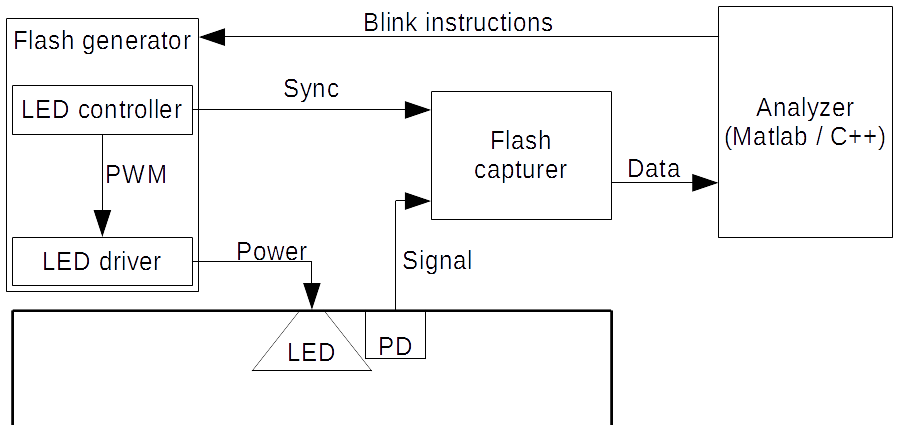
\includegraphics[width=\textwidth]{pics/systemOverview.png}
	\caption{System architecture of the created platform.\label{fig:systemOveriew}}
\end{figure}

\section{system components}

\subsection{Flash generator}
The flash generator is a device able to control a LED with high precision. It's able to set the period $T$, and the t-on time $T_{on}$. $T$ controls the frequency of the flashes and $T_{on}$ the length. Both parameters can be set with a resolution of $10\mu s$ resulting in a precisely controlled PWM signal with the help of equation \ref{eq:1/f=T}. This signal is sent to a LED driver through one of three LED drivers, which will make the actual light turn on and off at different light levels.

\begin{equation}
\label{eq:1/f=T}
T=\frac{1}{f}
\qquad
DutyCycle=\frac{T_{on}}{T} * 100\%
\end{equation}
Besides generating the PWM signal for the light, the flash generator has another function. It sends a sync signal to the flash receiver just before generating a flash. This allows the flash receiver to be ready when the flash starts, so it does not waste time sampling if no flash is generated.

\begin{figure}[]
	\centering
	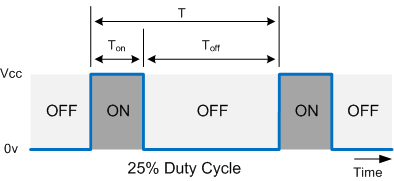
\includegraphics[]{pics/DutyCycle.png}
	\caption{Visualization of how $T$ and $T_{on}$ determine the duty cycle and frequency of the flash generator.\label{fig:DutyCycle}}
\end{figure}

\subsection{Reflection receiver}
The job of the receiver is to sample values while the light is being turned on and off, to then analyse the full reflected flash and extract a feature which properly represents the environment. The receiver should therefore capture flashes as precise and consistent as possible. For this reason, the receiver receives a sync signal from the flash generator and is therefore able to start sampling at almost the same moment every time, relative to the start of the flash. 

The receiver should continue sampling for a set period of time. Once done, the device should do one of the following things with the received samples, depending on the mode of the analyser:
\begin{enumerate}[itemsep=-1ex,topsep=0pt]
	\item Send back the full flash, uncompressed, for the analysis of separate flashes.
	\item Send back all compressed flashes, by extracting several features.
\end{enumerate}

\subsection{Analyser}
The analyser will receive samples from the reflection receiver and is ran on a PC in the form of either a C/C++ program (real-time) or as a MATLAB script (post-time). The analyser can set the receiver to work in \textit{raw} or \textit{compressed} mode. If the receiver sends raw flashes to the analyser it can be used to analyse these flashes in detail. This mode is used in chapter \ref{chp:Flash_Analysis} to analyse single flashes in order to find the ideal settings for the flash generator and reflection receiver. If the receiver sends compressed flashes, the analyser is able to analyse consecutive flashes. This mode will be used in chapter \ref{chp:Analyser} to find an algorithm to determine if an object is moving in the area under the light.

The Analyser should also be able to control the flash generator if the system is running in real-time mode. It is therefore able to send a packet with $T$, ${T_{on}}$ and $I_{LED}$ to the device. This allows for real time control of the flash generator.

\section{Implementation}
The system was build by combining several off shelf components. An overview of the actual platform can be seen in figure \ref{fig:acutalBuild}. It shows the different components mounted on a box. This section will explain briefly how each system component is implemented and why each part was chosen.

The flash generator is implemented on an Arduino UNO\cite{ArduinoUno}. This platform was chosen, as it's simple to use, does not require an operating system (OS) and has therefore no unexpected jitter. The LED used in the set-up is the same LED as modelled in chapter\ref{Model}. The power used by the LED is regulated with a single resistor. The resistors where chosen after some experimentation with the flash generation and reception. The values and resulting LED current can be seen in equation \ref{eq:Power}.

\begin{equation}
\label{eq:Power}
I_{LED}=\frac{V_{DD} - U_{LED}}{R}
\qquad
I_{LED} = \frac{7 - 3.6}{[1, 3, 5]} = [3.4A, 1.1A, 0.68A]
\end{equation}

The reflection receiver is implemented on the shine platform \cite{Shine}. This platform was chosen because it's a simple (no OS required) hands-on platform featuring multiple photodiodes by default. The original software of shine sampled each photodiode at 1Khz. This is way too low to see the $10\mu s$ flash resolution. For this reason the software of shine was rewritten to sample in bursts of 50 samples at 210Khz (for a total of$\pm 240\mu s$) when the sync signal is received.

A downside of the shine platform is that it's unable to communicate directly with the analyser as it does not has a FTDI interface. This problem was solved by using a processor-less Arduino UNO as bridge between the analyser and shine platform.

The receiver makes use of three photodiodes of which it will use one at a time. The original sensors on shine where replaced with ones more sensitive to visible light. Each sensor is configured in a different way. Some feature an increased amplification of the measured signal. Others have a longer wire with (intentional) bad shielding which can simulate how the system preforms in a environment with lots of electromagnetic radiation. An overview of the PD configurations can be seen in table \ref{tbl:PDs}.

Another important decision concerns the amplification circuit of the photodiode. The original circuit used by shine uses an analogue low-pass filter to remove ripple introduced by the amplifier (See Figure \ref{fig:FristFlashes}). The filter has several side effects. It reduces the signal strength and decreases the time the signal is visible to the system. It was therefore chosen to remove al analogue filters from shine and deal with the ripple with the help of software if required. The ripple effect might even be useful as the it's probably dependent on the received signal strength and therefore a measure of the environment.

\begin{table}[]
	\centering
	\begin{tabular}{clll}
		PD\#                   & Wire length & Gain  & EMC Shield \\ \cline{2-4} 
		\multicolumn{1}{c|}{1} & Long        & 1000  & Slecteable \\
		\multicolumn{1}{c|}{2} & Short       & 5600  & Yes        \\
		\multicolumn{1}{c|}{3} & Short       & 10000 & Yes       
	\end{tabular}
	\caption{Overview of photodiode configurations.\label{tbl:PDs}}
\end{table}

\begin{figure}
	\centering     %%% not \center
	\subfigure[Top view]{\label{fig:top}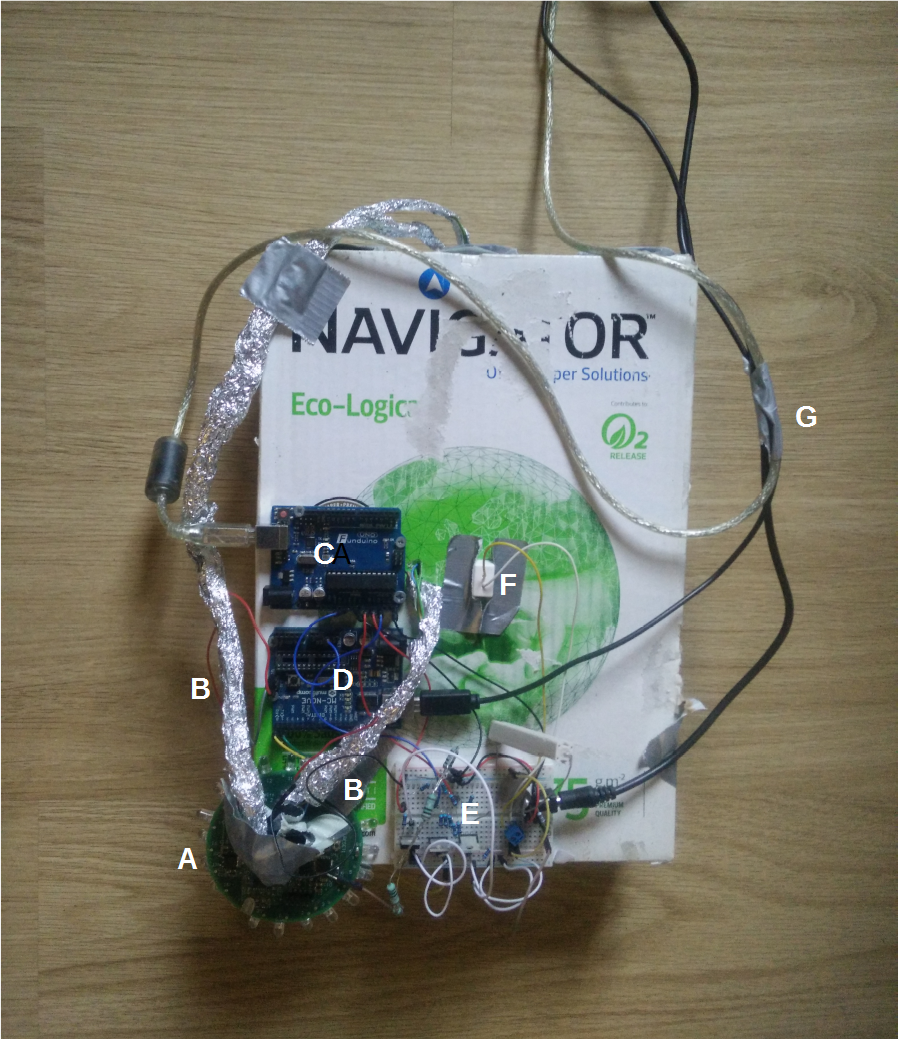
\includegraphics[width=60mm]{pics/platform_top.png}}
	\subfigure[Bottom view]{\label{fig:bot}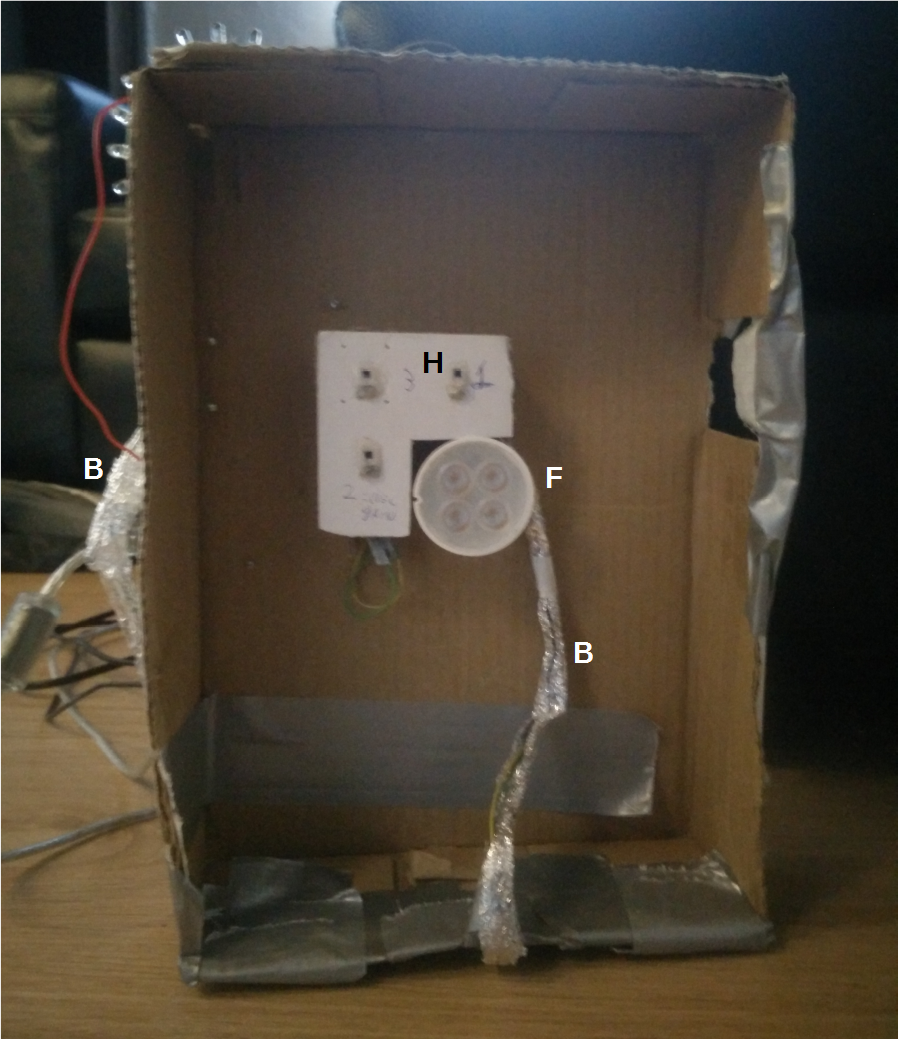
\includegraphics[width=60mm]{pics/platform_bot.png}}
	\captionsetup{singlelinecheck=off}
	\caption[]{The platform prototype. Each letter denotes a different component:
		\begin{enumerate}[label=\Alph*,itemsep=-1ex,topsep=0pt]
			\item = Reflection receiver
			\item = Wires to the photodiodes
			\item = LED controller
			\item = Communication bridge between shine and the PC
			\item = LED driver
			\item = The LED
			\item = Wires to the analyser and power supply
			\item = Three photodiodes
	    \end{enumerate}\label{fig:acutalBuild}}
\end{figure}

\section{Summary}
The system has been built and tested. Even though the created device has a poor build quality, it has great potential for experimentation with the proposed method of activity detection. The main advantages are:
\begin{itemize}[itemsep=-1ex]
	\item Each building block has one clear purpose and can therefore be tackled separately from other components. It's therefore impossible that a timing error in the flash generator software affects the sampling of the receiver or vice versa.
	\item The build quality is poor. If the project works on this device, it will definitely work on a dedicated platform.
\end{itemize}
The next steps for the project is finding a method for extracting useful information from flashes as shown in figure \ref{fig:notfiltered}. 

\begin{figure}
	\centering     %%% not \center
	\subfigure[Unfiltered flash]{\label{fig:notfiltered}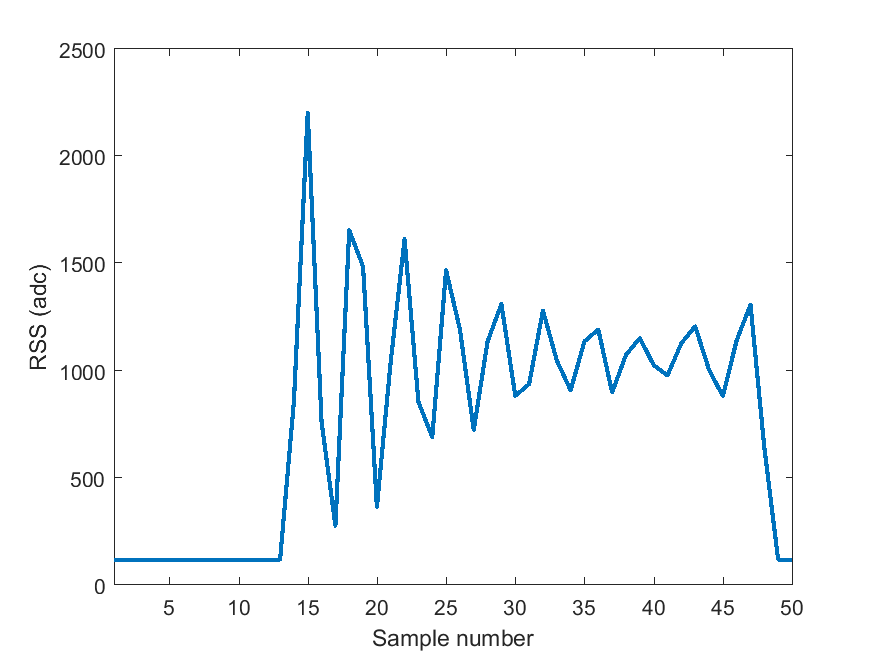
\includegraphics[width=60mm]{pics/no_filter.png}}
	\subfigure[Filtered flash]{\label{fig:filtered}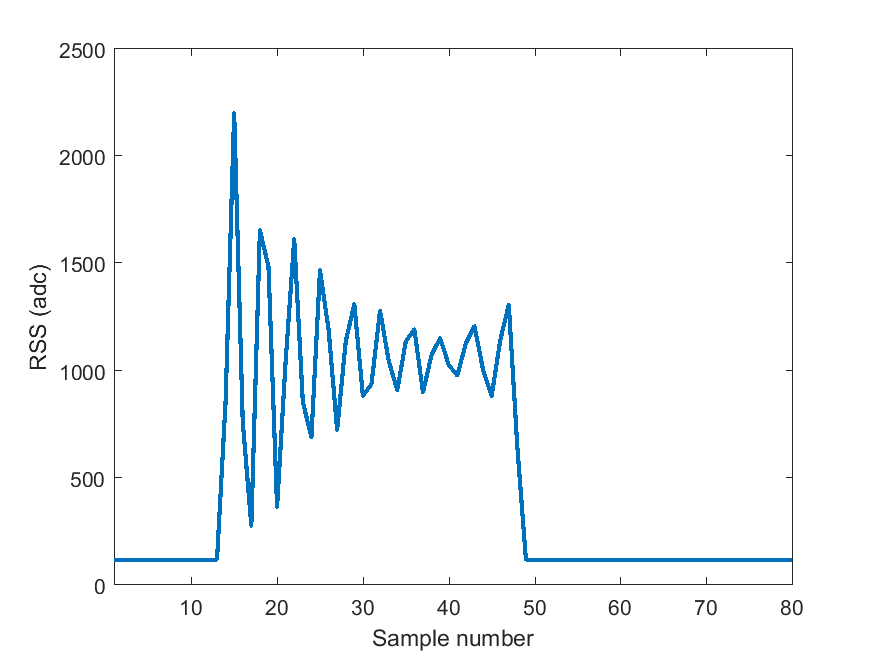
\includegraphics[width=60mm]{pics/analog_filter.png}}
	\caption{Two flashes captured with the platform. Left is unfiltered, right is filtered.	\label{fig:FristFlashes}}
\end{figure}